 % - Components and their Interfaces
 %   - Parent subnet node
 %   - Child subnet node
 %   - IPC module
 %   - Subnet actor
 \section{Components and their Interfaces}
 \label{sec:components}

We now focus on the interaction between two subnets in a parent-child relation.
To enable the interaction between them, which comprises running the subnets, observing each other's replicated state,
constructing \pofsFull, submitting the necessary transactions, and modifying the replicated state accordingly,
the following components need to work together.\\

\begin{itemize}
    \item Processes:
        \begin{enumerate}
            \item \textbf{Parent replica:} The process that runs the parent subnet. It has a copy of the parent's replicated state, participates in receiving and ordering transactions and updates the replicated state (including the \sa \dapp) accordingly.
            \item \textbf{Child replica:} The process that runs the child subnet. It has a copy of the child's replicated state, participates in receiving and ordering transactions and updates the replicated state (including the \gw \dapp) accordingly.
            \item \textbf{\ipc agent:} The process that mediates the interactions between the two subnets.
            It has access to the replicated states of both the parent and the child
            (e.g., by sharing a trust domain with a child and a parent replica, or by securely downloading the replicated state from other replicas...)
            and acts as an SMR client (i.e. submits transactions) to both subnets.
            Depending on the implementation, it might also be responsible for constructing \pofsFull (which might involve communication with other processes).
        \end{enumerate}
    \item Smart contracts:
        \begin{enumerate}
            \item \textbf{Subnet actor (\sa):} The smart contract in the parent subnet's replicated state
            that stores all information about the child subnet that the parent subnet needs.
            The \ipc agent's transactions submitted to the parent subnet mostly invoke the \sa.
            The state of the \sa includes:
            \begin{itemize}
            \item \emph{Accounting data.}
            This data describes the money that has been deposited to the child.
            It is considered locked inside the SA until it is withdrawn from the child.
            This data might consist of just a single value representing the sum of all such coins ("custodial" approach),
            but might also contain finer-grained information about balances for each account in the child subnet ("non-custodial" approach).
            %We continue with the non-custodial approach as the other can be viewed as a specific limitation of it.
            \item \emph{Governance account.}
            This account facilitates the economic design of a subnet.
            It can be used for collecting fees or making payments to accounts of participants that perform operations on behalf of the child subnet.
            For example, when an IPC agent submits (and thus pays for) transaction linking a child's checkpoint to the parent's replicated state,
            the IPC actor logic might reimburse the associated account.
            \item \emph{Ordering protocol data.}
            This is the data (or a pointer to it) that is needed to run the ordering protocol of the child subnet.
            It is protocol-specific, but is generally expected to contain information such as
            \begin{itemize}
                \item The ordering protocol used by the subnet.
                \item Subnet configuration such as the validator set, voting rights, collateral deposits, etc.
                \item Subnet governance mechanisms, e.g., transaction fees, block rewards, conditions for participation, ...
            \end{itemize}
            \item \emph{Child state finality verification.} Logic to verify (based on only the parent's replicated state)
            that a given child's replicated state/\tx is final%
\footnote{Finality is an elusive concept that we do not take upon ourselves to define here. For simplicity, we assume finality in a Boolean manner, either \tx is final or it is not. This could easily be generalized to parameterized finality of the sort ``the probability of \tx persisting is at least~$x$."}
            or that a particular \tx has been definitively included in the child's state.
            We expect that this logic will verify a \pof submitted (through transactions) by one or more IPC agents to the \sa.
            % For this, we will use the function \sa.\verifyGfinal{\tx}{\prf} which excepts as arguments a transaction (or state) and a \prf, and outputs True if \tx is considered globally final in the child subnet and False otherwise. This function must only depend on its inputs and the internal state of~\sa. For example, \prf is a threshold signature that can be verified against the set of validators in~\sa.
          
        \end{itemize}
        The above suffices for an \ipcFull system with a minimal inter-subnet functionality of users' asset transfer, and a general \smr per subnet. We continue with further state required for additional functionality.
        \begin{itemize}
            \item \emph{Slashing.}
            \begin{itemize}
                \item List of slashable misbehaviors and a proving methodology. That is, for each slashable misbehavior there is a definition of what constitutes a valid proof of misbehavior (\pom).
                \item Penalties for misbehavior and rewards for reporting, as well as the logic performing the necessary actions within the parent subnet.
            \end{itemize}
            \item \emph{Checkpointing.}
            \begin{itemize}
                \item Child subnet's checkpoint data or a pointer to it.
                \item Checkpoint validity rules (and logic enforcing them).
                E.g., "Checkpoints must be at least every~$\Delta$ subnet blocks apart", or "A checkpoint must contain a reference to (hash of) a previous checkpoint.", etc.
                % the checkpoint's $L_2$ distance from the previous is larger than~$L$.
                %\item Fee payments for checkpoints.
            \end{itemize}
        \end{itemize}
        \item \textbf{IPC coordinator/gateway actor (\gw):} a smart contract that exists in every subnet in the \ipc hierarchy and contains all information and logic the subnet itself needs to hold in order to be part of \ipc. The state of the \gw includes:
        \begin{itemize}
            \item \emph{Parent state finality verification.} Analogously to the \sa's child state finality verification logic,
            this is the logic to verify that a state/\tx is final in the parent subnet,
            using a \pof submitted as transaction(s) to the child subnet by the IPC agent(s).
            % For this, we will use the function \gw.\verifyPfinal{\tx}{\prf} which excepts as arguments a transaction (or state) and a \prf, and outputs True if \tx is considered globally final in the parent subnet and False otherwise. This function must only depend on its inputs (and perhaps some internal state of~\gw).
            \item \emph{Inter-subnet transactions service} (denoted \postoffice).
            The \gw contains a registry of subnets and a functionality that can be used to transfer data from one subnet to another. 
            The \postoffice specifies the methods and the state locations that are used for these services.
            This functionality is required for the communication of two smart contracts across subnets%
            % In particular, consider the following case involving a smart contract.%
\footnote{When inter-subnet data transfer happens between users (Externally Owned Accounts --- \eoa --- in Ethereum's jargon), they can actively participate in the propagation by submitting transactions to the parent and child subnets. Smart contracts, on the other hand, do not have that power and, therefore, cannot communicate inter-subnets as efficiently as users (\eoa) and must do so through IPC agents.},
            i.e., a smart contract emiting an event that contains data to be processed by the replicated state machine logic of a different subnet.
        \end{itemize}
    \end{enumerate}
\end{itemize}

% OLD VERSION:
% \begin{enumerate}
%     \item \textbf{\ipc agent:} The software that is in charge of the interactions between the two blockchains. This includes, for example, observers for the parent and child subnets. (Note that it is a process and not a smart contract). The \ipc agent is a piece of software that mediates the interactions between the child and parent \smr software modules.    
%     \item \textbf{Parent \smr replica:} The software that runs the parent blockchain. Note that this module also entails the interaction with the \ipc smart contract~\sa, which is maintained at the parent subnet. Any update that the parent process performs on \sa is notified to the \ipc agent.
%     \item \textbf{Child \smr replica:} The software that runs the child blockchain. Note that some of the rules the child blockchain must satisfy are listed in~\sa. Any output operation (withdraw, checkpoint) is notified to the parent process through the \ipc agent. 
% %    \item \textbf{IPC smart contract / subnet actor (\sa):} The smart contract implementation that is running on the parent blockchain. It is invoked only through transactions that are included in the parent blockchain.
%     \item \textbf{IPC subnet actor (\sa):} The smart contract implementation that is running on the parent blockchain. It is invoked only through transactions that are included in the parent blockchain.
%     \item \textbf{IPC coordinator/gateway actor (\gw):} a smart contract that exists in every non-leaf subnet in the \ipc hierarchy and contains methods facilitating inter-subnet operations.	
% \end{enumerate}


We now define minimal interfaces between the different modules that enable the correct operation of an \ipcFull system.
A guiding principle in the interface design is to minimize changes to the \smr codebase; therefore, most extra logic of the \ipc will be added into the \ipc agent and the smart contracts \sa~and~\gw. Doing so should facilitate the deployment of \ipc with new \smr protocols by not requiring a developer familiar with \ipc to be an expert on \smr: some understanding is still needed to optimize the agent's implementation, but the \smr code would remain portable.

We require four interfaces: (i) \ipc agent --- parent \smr, (ii) \ipc agent --- child \smr, (iii) parent \smr --- \sa, and (iv) any \smr --- \gw. Both (i) and (ii) can comprise of only:
\begin{enumerate}
    \item Agent submits a transaction~\tx to the \smr process.%
    \footnote{As part of the notification defined below, it could be that after submitting \tx, until the \smr process returns \textit{complete} (perhaps with a finality parameter) or \textit{declined}, \tx is considered \textit{pending}.}
    \item Agent queries the state of the \smr process. The \smr process returns its current state (possibly limited to only a requested part of the state).
    \item \smr process notifies the agent on events of interest (e.g., changes to the state of~\sa).
\end{enumerate}

The interface between an \smr and~\sa or~\gw is based on the execution engine of that \smr and the functionality desired by~\sa. The specifics of the execution engine's system calls depend on implementation. Whenever such a call is not clear from context we provide a description of what it entails. \\

\Cref{fig:interfaces} illustrates the components and their interfaces.\\

\begin{figure}[h]
     \centering
     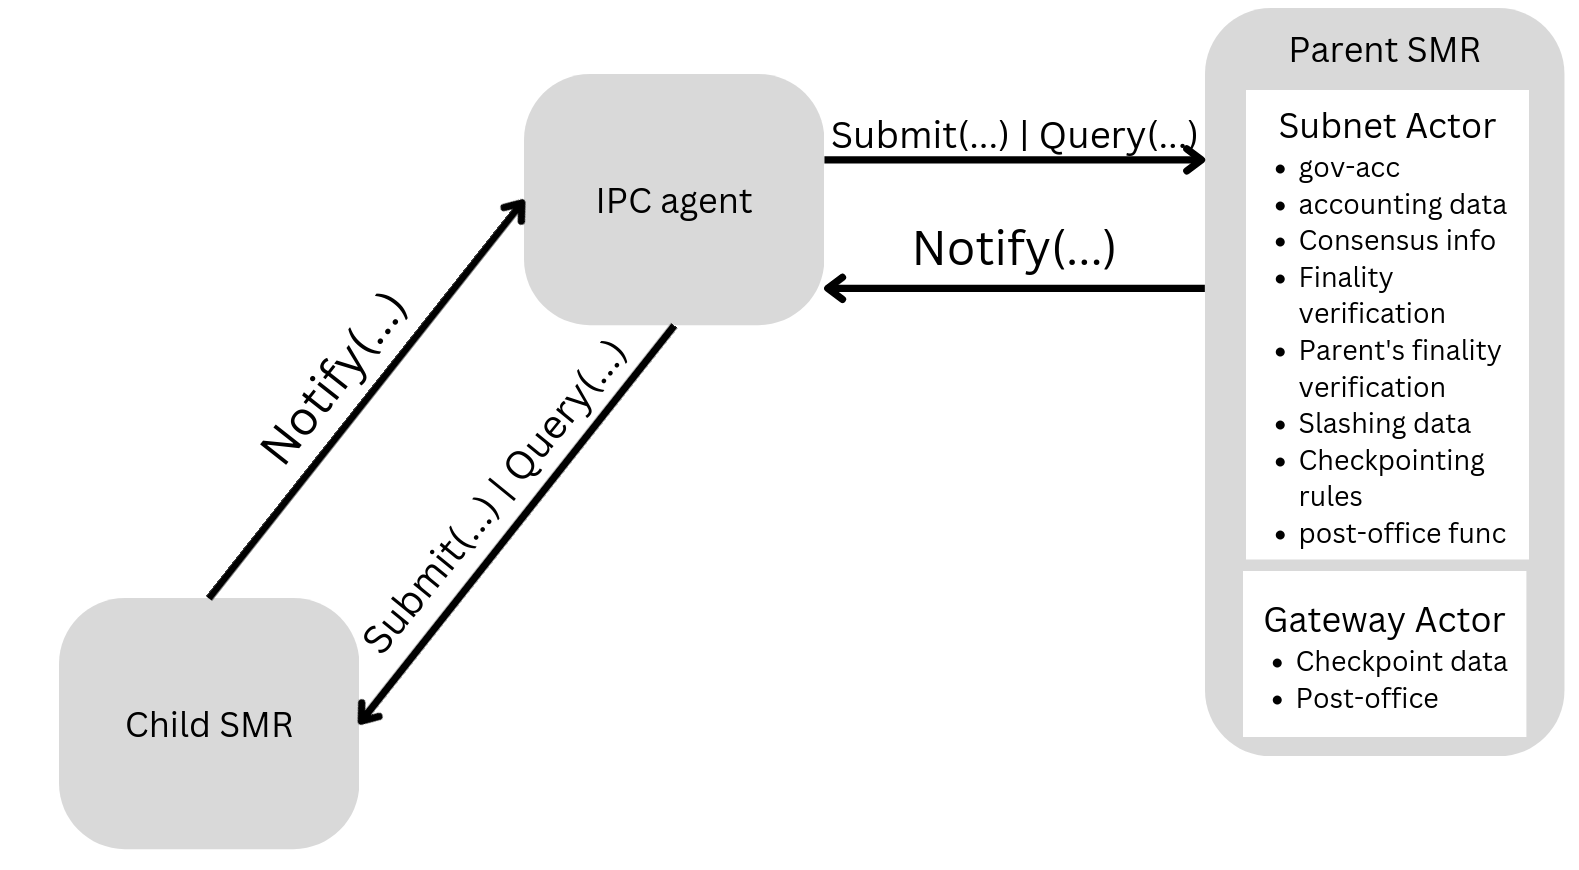
\includegraphics[width=0.75\textwidth]{compsintfs}
     \caption{The basic components and their interfaces.}
     \label{fig:interfaces}
 \end{figure}
